% !TeX program = xelatex
% Extended abstract, Agent Evaluation Science symposium (2 pages excl. references).
% Build: cd paper/abstract && latexmk -xelatex main.tex
% Numbers come from ../../analysis/tables/numbers.tex (python -m src.report);
% never type a result into the prose. "% CHECK" marks sentences to re-read
% against the final numbers once all runs are scored.
\documentclass[11pt,a4paper]{article}
\usepackage{aes}
\usepackage{tabularx}
\usepackage{tikz}
\usetikzlibrary{arrows.meta,calc}

\graphicspath{{../../analysis/figures/}}
% Generated by src/report.py from analysis/results/. Do not edit by hand.
\newcommand{\nWorkshopsSmall}{30}
\newcommand{\nCallsSmall}{2,420}
\newcommand{\pctAnsweredSmall}{98.7\%}
\newcommand{\nCardsSmall}{360}
\newcommand{\blockCardsSmall}{2}
\newcommand{\nWorkshopsLarge}{120}
\newcommand{\nCallsLarge}{16,699}
\newcommand{\pctAnsweredLarge}{99.9\%}
\newcommand{\nCardsLarge}{1440}
\newcommand{\blockCardsLarge}{2}
\newcommand{\nWorkshopsFull}{60}
\newcommand{\nCallsFull}{13,353}
\newcommand{\pctAnsweredFull}{99.9\%}
\newcommand{\nCardsFull}{720}
\newcommand{\blockCardsFull}{2}
\newcommand{\nWorkshopsAll}{150}
\newcommand{\nCallsAll}{19,119}
\newcommand{\pctAnsweredAll}{99.7\%}
\newcommand{\nCardsAll}{1800}
\newcommand{\blockCardsAll}{4}
\newcommand{\nRuns}{10}
\newcommand{\chanceRules}{1.66}
\newcommand{\chanceSpec}{6.38}
\newcommand{\chanceDecision}{14\%}
\newcommand{\rulesQwenSmall}{3.5}
\newcommand{\rulesRangeQwenSmall}{2--4}
\newcommand{\specQwenSmall}{6.4}
\newcommand{\decisionQwenSmall}{4/10}
\newcommand{\modalQwenSmall}{6/10}
\newcommand{\recallGapQwenSmall}{-4.6}
\newcommand{\blockQwenSmall}{0/10}
\newcommand{\moreSupportiveQwenSmall}{47}
\newcommand{\moreCriticalQwenSmall}{43}
\newcommand{\rulesGemmaSmall}{2.8}
\newcommand{\rulesRangeGemmaSmall}{2--3}
\newcommand{\specGemmaSmall}{0.9}
\newcommand{\decisionGemmaSmall}{6/10}
\newcommand{\modalGemmaSmall}{6/10}
\newcommand{\recallGapGemmaSmall}{+1.1}
\newcommand{\blockGemmaSmall}{0/10}
\newcommand{\moreSupportiveGemmaSmall}{119}
\newcommand{\moreCriticalGemmaSmall}{0}
\newcommand{\rulesMistralSmall}{2.4}
\newcommand{\rulesRangeMistralSmall}{1--4}
\newcommand{\specMistralSmall}{5.4}
\newcommand{\decisionMistralSmall}{1/10}
\newcommand{\modalMistralSmall}{7/10}
\newcommand{\recallGapMistralSmall}{+6.5}
\newcommand{\blockMistralSmall}{2/10}
\newcommand{\moreSupportiveMistralSmall}{115}
\newcommand{\moreCriticalMistralSmall}{0}
\newcommand{\rulesQwenLargeLite}{1.45}
\newcommand{\rulesRangeQwenLargeLite}{1--3}
\newcommand{\specQwenLargeLite}{6.55}
\newcommand{\decisionQwenLargeLite}{0/20}
\newcommand{\modalQwenLargeLite}{20/20}
\newcommand{\recallGapQwenLargeLite}{+6.1}
\newcommand{\blockQwenLargeLite}{0/20}
\newcommand{\moreSupportiveQwenLargeLite}{108}
\newcommand{\moreCriticalQwenLargeLite}{85}
\newcommand{\rulesGemmaLargeLite}{1.0}
\newcommand{\rulesRangeGemmaLargeLite}{1--1}
\newcommand{\specGemmaLargeLite}{5.4}
\newcommand{\decisionGemmaLargeLite}{0/20}
\newcommand{\modalGemmaLargeLite}{20/20}
\newcommand{\recallGapGemmaLargeLite}{+6.1}
\newcommand{\blockGemmaLargeLite}{0/20}
\newcommand{\moreSupportiveGemmaLargeLite}{213}
\newcommand{\moreCriticalGemmaLargeLite}{27}
\newcommand{\rulesMistralLargeLite}{2.5}
\newcommand{\rulesRangeMistralLargeLite}{2--4}
\newcommand{\specMistralLargeLite}{5.9}
\newcommand{\decisionMistralLargeLite}{3/20}
\newcommand{\modalMistralLargeLite}{16/20}
\newcommand{\recallGapMistralLargeLite}{+4.5}
\newcommand{\blockMistralLargeLite}{0/20}
\newcommand{\moreSupportiveMistralLargeLite}{83}
\newcommand{\moreCriticalMistralLargeLite}{22}
\newcommand{\rulesQwenLargeFull}{1.9}
\newcommand{\rulesRangeQwenLargeFull}{1--3}
\newcommand{\specQwenLargeFull}{6.8}
\newcommand{\decisionQwenLargeFull}{0/20}
\newcommand{\modalQwenLargeFull}{20/20}
\newcommand{\recallGapQwenLargeFull}{+6.1}
\newcommand{\blockQwenLargeFull}{2/20}
\newcommand{\moreSupportiveQwenLargeFull}{11}
\newcommand{\moreCriticalQwenLargeFull}{215}
\newcommand{\rulesGemmaLargeFull}{1.35}
\newcommand{\rulesRangeGemmaLargeFull}{1--3}
\newcommand{\specGemmaLargeFull}{5.45}
\newcommand{\decisionGemmaLargeFull}{0/20}
\newcommand{\modalGemmaLargeFull}{20/20}
\newcommand{\recallGapGemmaLargeFull}{+6.1}
\newcommand{\blockGemmaLargeFull}{0/20}
\newcommand{\moreSupportiveGemmaLargeFull}{1}
\newcommand{\moreCriticalGemmaLargeFull}{239}
\newcommand{\rulesMistralLargeFull}{3.1}
\newcommand{\rulesRangeMistralLargeFull}{2--4}
\newcommand{\specMistralLargeFull}{5.5}
\newcommand{\decisionMistralLargeFull}{3/20}
\newcommand{\modalMistralLargeFull}{14/20}
\newcommand{\recallGapMistralLargeFull}{+3.1}
\newcommand{\blockMistralLargeFull}{0/20}
\newcommand{\moreSupportiveMistralLargeFull}{145}
\newcommand{\moreCriticalMistralLargeFull}{23}
\newcommand{\sizeDiffQwen}{-2.05}
\newcommand{\sizeCIQwen}{[-2.50, -1.55]}
\newcommand{\protocolDiffQwen}{+0.45}
\newcommand{\protocolCIQwen}{[+0.05, +0.80]}
\newcommand{\sizeDiffGemma}{-1.80}
\newcommand{\sizeCIGemma}{[-2.00, -1.50]}
\newcommand{\protocolDiffGemma}{+0.35}
\newcommand{\protocolCIGemma}{[+0.10, +0.65]}
\newcommand{\sizeDiffMistral}{+0.10}
\newcommand{\sizeCIMistral}{[-0.55, +0.75]}
\newcommand{\protocolDiffMistral}{+0.60}
\newcommand{\protocolCIMistral}{[+0.20, +0.95]}
\newcommand{\nRunsLarge}{120}
\newcommand{\lrcLarge}{110}
\newcommand{\enrolLowLarge}{110}
\newcommand{\humanSelfRules}{3}
\newcommand{\humanSelfSpec}{10}
\newcommand{\humanChangedRules}{4}
\newcommand{\shiftItemsQwenSmall}{5.5}
\newcommand{\shiftStricterQwenSmall}{2.0}
\newcommand{\shiftPermissiveQwenSmall}{3.5}
\newcommand{\rulesShiftedQwenSmall}{1.8}
\newcommand{\shiftSameQwenSmall}{10\%}
\newcommand{\shiftItemsGemmaSmall}{5.3}
\newcommand{\shiftStricterGemmaSmall}{1.6}
\newcommand{\shiftPermissiveGemmaSmall}{3.7}
\newcommand{\rulesShiftedGemmaSmall}{1.6}
\newcommand{\shiftSameGemmaSmall}{7\%}
\newcommand{\shiftItemsMistralSmall}{5.7}
\newcommand{\shiftStricterMistralSmall}{2.0}
\newcommand{\shiftPermissiveMistralSmall}{3.7}
\newcommand{\rulesShiftedMistralSmall}{2.3}
\newcommand{\shiftSameMistralSmall}{11\%}
\newcommand{\shiftItemsQwenLargeLite}{2.5}
\newcommand{\shiftStricterQwenLargeLite}{1.4}
\newcommand{\shiftPermissiveQwenLargeLite}{1.1}
\newcommand{\rulesShiftedQwenLargeLite}{1.0}
\newcommand{\shiftSameQwenLargeLite}{3\%}
\newcommand{\shiftItemsGemmaLargeLite}{0.9}
\newcommand{\shiftStricterGemmaLargeLite}{0.0}
\newcommand{\shiftPermissiveGemmaLargeLite}{0.9}
\newcommand{\rulesShiftedGemmaLargeLite}{0.0}
\newcommand{\shiftSameGemmaLargeLite}{0\%}
\newcommand{\shiftItemsMistralLargeLite}{3.0}
\newcommand{\shiftStricterMistralLargeLite}{1.4}
\newcommand{\shiftPermissiveMistralLargeLite}{1.6}
\newcommand{\rulesShiftedMistralLargeLite}{1.3}
\newcommand{\shiftSameMistralLargeLite}{5\%}
\newcommand{\shiftItemsQwenLargeFull}{4.2}
\newcommand{\shiftStricterQwenLargeFull}{3.7}
\newcommand{\shiftPermissiveQwenLargeFull}{0.5}
\newcommand{\rulesShiftedQwenLargeFull}{2.8}
\newcommand{\shiftSameQwenLargeFull}{15\%}
\newcommand{\shiftItemsGemmaLargeFull}{1.8}
\newcommand{\shiftStricterGemmaLargeFull}{0.7}
\newcommand{\shiftPermissiveGemmaLargeFull}{1.1}
\newcommand{\rulesShiftedGemmaLargeFull}{0.1}
\newcommand{\shiftSameGemmaLargeFull}{0\%}
\newcommand{\shiftItemsMistralLargeFull}{2.2}
\newcommand{\shiftStricterMistralLargeFull}{1.4}
\newcommand{\shiftPermissiveMistralLargeFull}{0.8}
\newcommand{\rulesShiftedMistralLargeFull}{1.0}
\newcommand{\shiftSameMistralLargeFull}{4\%}
\newcommand{\humanShiftItems}{10}
\newcommand{\humanShiftStricter}{7}
\newcommand{\humanShiftPermissive}{3}
\newcommand{\humanSensitiveStricter}{5}
\newcommand{\nSensitive}{7}
\newcommand{\nRunsFullAll}{60}
\newcommand{\lrcFull}{54}
\newcommand{\enrolLowFull}{54}
\newcommand{\baseLrcFull}{58}
\newcommand{\supportCardsFull}{0}
\newcommand{\humanSupportCards}{4}
\newcommand{\humanSupportWithReservationsCards}{2}
\newcommand{\humanObjectNoBlockCards}{2}
\newcommand{\humanBlockCards}{2}
\newcommand{\reservationsFull}{97\%}
\newcommand{\changedQwenSmall}{23\%}
\newcommand{\changedGemmaSmall}{20\%}
\newcommand{\changedMistralSmall}{29\%}
\newcommand{\changedQwenLargeLite}{10\%}
\newcommand{\changedGemmaLargeLite}{3\%}
\newcommand{\changedMistralLargeLite}{13\%}
\newcommand{\changedQwenLargeFull}{13\%}
\newcommand{\changedGemmaLargeFull}{3\%}
\newcommand{\changedMistralLargeFull}{7\%}
% aliases: small tier
\newcommand{\rulesQwen}{\rulesQwenSmall}
\newcommand{\rulesRangeQwen}{\rulesRangeQwenSmall}
\newcommand{\specQwen}{\specQwenSmall}
\newcommand{\decisionQwen}{\decisionQwenSmall}
\newcommand{\modalQwen}{\modalQwenSmall}
\newcommand{\recallGapQwen}{\recallGapQwenSmall}
\newcommand{\blockQwen}{\blockQwenSmall}
\newcommand{\moreSupportiveQwen}{\moreSupportiveQwenSmall}
\newcommand{\moreCriticalQwen}{\moreCriticalQwenSmall}
\newcommand{\rulesGemma}{\rulesGemmaSmall}
\newcommand{\rulesRangeGemma}{\rulesRangeGemmaSmall}
\newcommand{\specGemma}{\specGemmaSmall}
\newcommand{\decisionGemma}{\decisionGemmaSmall}
\newcommand{\modalGemma}{\modalGemmaSmall}
\newcommand{\recallGapGemma}{\recallGapGemmaSmall}
\newcommand{\blockGemma}{\blockGemmaSmall}
\newcommand{\moreSupportiveGemma}{\moreSupportiveGemmaSmall}
\newcommand{\moreCriticalGemma}{\moreCriticalGemmaSmall}
\newcommand{\rulesMinistral}{\rulesMistralSmall}
\newcommand{\rulesRangeMinistral}{\rulesRangeMistralSmall}
\newcommand{\specMinistral}{\specMistralSmall}
\newcommand{\decisionMinistral}{\decisionMistralSmall}
\newcommand{\modalMinistral}{\modalMistralSmall}
\newcommand{\recallGapMinistral}{\recallGapMistralSmall}
\newcommand{\blockMinistral}{\blockMistralSmall}
\newcommand{\moreSupportiveMinistral}{\moreSupportiveMistralSmall}
\newcommand{\moreCriticalMinistral}{\moreCriticalMistralSmall}
\newcommand{\nWorkshops}{\nWorkshopsSmall}
\newcommand{\nCalls}{\nCallsSmall}
\newcommand{\pctAnswered}{\pctAnsweredSmall}
\newcommand{\nCards}{\nCardsSmall}
\newcommand{\blockCards}{\blockCardsSmall}


\title[Synthetic Stakeholders?]{Synthetic Stakeholders? Validity and Stability of Open-Weight LLM Agent Panels in Participatory Model Selection}

\aesauthor[affil={1},corresponding]{Tereza Bla\v{z}kov\'a}
\aesaffiliation{1}{[Affiliation, TODO]}
\aesemails{\aesemail{[email, TODO]}}

\begin{document}
\maketitle

\begin{abstract}
LLM agents are proposed as synthetic participants, but rarely tested against a real participatory deliberation.
We replicate a workshop in which 12 students and advisors set the rules for selecting a university dropout early-warning model, with 12-agent panels from three small open-weight model families (\nRuns{} workshops each), and apply each panel's median rules to the same candidate models.
Panels recovered on average \rulesQwen{}, \rulesGemma{} and \rulesMinistral{} of the 7 human selection rules (Qwen, Gemma, Ministral; random panels: \chanceRules{}) and selected the human-chosen model in \decisionQwen{}, \decisionGemma{} and \decisionMinistral{} runs, but the family that chose it most often did so through rules the humans rejected, and panels almost never objected (\blockCards{} blocking votes in \nCards{}), suggesting that small synthetic panels can rehearse but not replace stakeholder deliberation.
\end{abstract}

\section{Motivation}
Participatory AI asks affected people to shape algorithmic systems \citep{birhanePowerPeopleOpportunities2022,delgadoParticipatoryTurnAI2023}; because this is slow and costly, LLM-simulated respondents are proposed as a substitute \citep{argyle2023outofone,aher2023using}, despite evidence that they misrepresent and flatten the groups they stand in for \citep{santurkar2023whose,wang2025misportray}.
We evaluate synthetic panels on what participation \emph{produces}: binding rules and the model they select.

\begin{figure}[b]
  \centering
  % Design diagram: the human workshop (top lane) and a synthetic panel (bottom
% lane) pass through the same stages. The two are compared at the baseline and
% at the endline survey (and on the change between them). The grey stages are
% not part of the simulated workshop: the endline medians are turned into rules
% and a model programmatically, identically in both lanes.
% Edit labels freely; layout is a 6-column grid.
\begin{tikzpicture}[
    font=\scriptsize,
    stage/.style={rectangle, rounded corners=2pt, align=center, minimum height=9mm,
                  text width=20mm, inner sep=1.5pt, draw=#1!75!black, fill=#1!10, line width=0.5pt,
                  execute at begin node={\hyphenpenalty=10000\relax}},
    derived/.style={rectangle, rounded corners=2pt, align=center, minimum height=9mm,
                  text width=20mm, inner sep=1.5pt, draw=black!30, fill=black!4, text=black!55,
                  line width=0.5pt, dashed, execute at begin node={\hyphenpenalty=10000\relax}},
    flow/.style={-{Stealth[length=1.5mm]}, line width=0.5pt, draw=black!50},
    gflow/.style={-{Stealth[length=1.5mm]}, line width=0.5pt, draw=black!25},
    cmp/.style={{Stealth[length=1.6mm]}-{Stealth[length=1.6mm]}, line width=0.9pt, draw=black},
    cmplabel/.style={font=\tiny\bfseries, fill=white, inner sep=1pt, align=center},
    lane/.style={font=\scriptsize\bfseries, anchor=east, align=right},
    note/.style={font=\tiny, text=black!60, fill=white, inner sep=1pt, align=center},
  ]
  \def\dx{22.5mm}
  \def\dy{15mm}
  \colorlet{hum}{black!45}
  \colorlet{syn}{aespurple}

  % ---- human lane ----
  \node[stage=hum] (h1) at (0,0)      {9 students\\+ 3 advisors};
  \node[stage=hum] (h2) at (\dx,0)    {Baseline survey};
  \node[stage=hum] (h3) at (2*\dx,0)  {3\,h deliberation};
  \node[stage=hum] (h4) at (3*\dx,0)  {Endline survey};
  \node[derived] (h5) at (4*\dx,0)    {Median rules};
  \node[derived] (h6) at (5*\dx,0)    {Logistic regression\\+ performance};

  % ---- synthetic lane ----
  \node[stage=syn] (s1) at (0,-\dy)     {12 LLM agents\\(fictional personas)};
  \node[stage=syn] (s2) at (\dx,-\dy)   {Baseline survey};
  \node[stage=syn] (s3) at (2*\dx,-\dy) {same protocol\\(scripted)};
  \node[stage=syn] (s4) at (3*\dx,-\dy) {Endline survey};
  \node[derived] (s5) at (4*\dx,-\dy)   {Median rules};
  \node[derived] (s6) at (5*\dx,-\dy)   {Selected model};

  \foreach \i/\j in {1/2,2/3,3/4} {
    \draw[flow] (h\i) -- (h\j);
    \draw[flow] (s\i) -- (s\j);
  }
  \foreach \i/\j in {4/5,5/6} {
    \draw[gflow] (h\i) -- (h\j);
    \draw[gflow] (s\i) -- (s\j);
  }

  % the comparisons: the same survey, before and after deliberation
  \draw[cmp] (h2.south) -- node[cmplabel] {compare\\baseline} (s2.north);
  \draw[cmp] (h4.south) -- node[cmplabel] {compare\\endline} (s4.north);

  % lane labels, the manipulated factor, the programmatic (not simulated) steps
  \node[lane, text=black!70] at ($(h1.west)+(-1.5mm,0)$) {Human\\workshop};
  \node[lane, text=aespurple!80!black] at ($(s1.west)+(-1.5mm,0)$) {Synthetic\\panel};
  \node[note, text=aespurple!80!black, anchor=north] at ($(s2.south)!0.5!(s4.south)+(0,-0.8mm)$)
       {3 open-weight families (Qwen 3.5 27B, Gemma 3 27B, Mistral Small 3.2 24B) $\times$ 20 seeded runs};
  \node[note, text=black!50, anchor=south] at ($(h5.north)!0.5!(h6.north)+(0,0.8mm)$)
       {not simulated: same median rule and selection algorithm in both lanes};
\end{tikzpicture}

  \caption{Design. Synthetic panels pass through the same survey, aggregation and selection algorithm as the human workshop; the model family is the only manipulated factor.}
  \label{fig:design}
\end{figure}

\section{Ground truth and design}
In a three-hour deliberative workshop at a Danish university \citep{blazkova2026participatory}, 9 students and 3 student advisors answered a survey before and after deliberation \citep{fishkin2009people}, pricing each step on two ladders in students identified per 100: adding data (course performance, enrolment, LMS activity, sensitive attributes) and lowering explainability (from a credit rule to a neural network).
Their endline medians, applied to all candidate models on the 2021 cohort, selected logistic regression on credits and performance (recall 62.3\% vs.\ 23.5\% for the current credit rule).
Because the human pre-deliberation rules select the same model, rule agreement is our main validity outcome.
Synthetic panels replay this process (Figure~\ref{fig:design}): 12 fictional personas with the published role and demographic mix, the verbatim survey, a scripted facilitator, one plenary round (seeded order, matched across families) and a final acceptability card.
The only manipulated factor is the model family: Qwen 3.5 4B, Gemma 3 4B and Ministral 3 3B (4-bit, local, temperature~1).
The scoring checklist and a random-panel reference were fixed before any model output; no personal data or transcripts were used, and \pctAnswered{} of choice items were answered (\nWorkshops{} workshops, \nCalls{} calls).

\section{Results}
\begin{figure}[t]
  \centering
  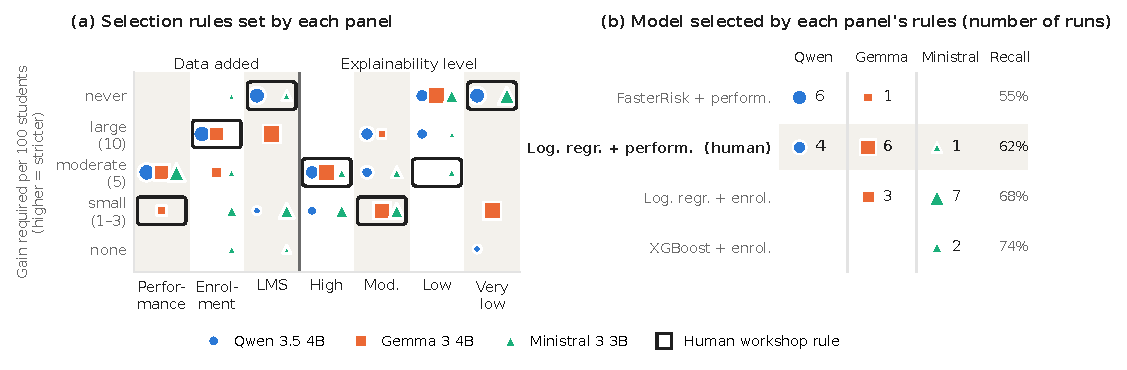
\includegraphics[width=\linewidth]{fig_rules.pdf}
  \caption{(a)~Selection rules set by each panel (endline medians; marker area = runs) against the human rules (boxes): above a box is stricter, below more permissive. (b)~Configuration selected by each panel's rules (runs) and its 2021 recall; the human choice is shaded.}
  \label{fig:agreement}
\end{figure}

\begin{table}[t]
  \centering\footnotesize
  \begin{tabular}{@{}llccccr@{}}
\toprule
Setting & Model & Rules /7 & Other /16 & Human model [95\% CI] & Modal & Recall gap \\
\midrule
small, lite & Qwen 3.5 4B & 3.5 (2--4) & 6.4 & 4/10 [.17--.69] & 6/10 & -4.6 pp \\
small, lite & Gemma 3 4B & 2.8 (2--3) & 0.9 & 6/10 [.31--.83] & 6/10 & +1.1 pp \\
small, lite & Ministral 3 3B & 2.4 (1--4) & 5.4 & 1/10 [.02--.40] & 7/10 & +6.5 pp \\
\midrule
large, lite & Qwen 3.5 27B & 1.45 (1--3) & 6.55 & 0/20 [.00--.16] & 20/20 & +6.1 pp \\
large, lite & Gemma 3 27B & 1.0 (1--1) & 5.4 & 0/20 [.00--.16] & 20/20 & +6.1 pp \\
large, lite & Mistral Small 3.2 24B & 2.5 (2--4) & 5.9 & 3/20 [.05--.36] & 16/20 & +4.5 pp \\
\midrule
large, full & Qwen 3.5 27B & 1.9 (1--3) & 6.8 & 0/20 [.00--.16] & 20/20 & +6.1 pp \\
large, full & Gemma 3 27B & 1.35 (1--3) & 5.45 & 0/20 [.00--.16] & 20/20 & +6.1 pp \\
large, full & Mistral Small 3.2 24B & 3.1 (2--4) & 5.5 & 3/20 [.05--.36] & 14/20 & +3.1 pp \\
\midrule
Random panel & & 1.66 & 6.38 & 14\% & -- & -- \\
\bottomrule
\end{tabular}

  \caption{Rules matched of 7 (range), other assessed items of 16, runs selecting the human model [Wilson 95\% CI] or the modal configuration, recall gap, items unanswered per workshop.}
  \label{tab:main}
\end{table}

All three families recover more selection rules than random panels, but at most half of them, and none beats random panels on the 16 other assessed items (Figure~\ref{fig:agreement}, Table~\ref{tab:main}).
The families err in different directions: Qwen panels are stricter about explainability and mostly select an integer scorecard (recall gap \recallGapQwen{}~pp), while Ministral panels accept enrolment data the humans priced high and select a more accurate model (\recallGapMinistral{}~pp).
Gemma panels select the human model most often (\decisionGemma{}), yet declare LMS data and neural networks acceptable, which the humans ruled out: the right decision from different rules.
The modal configuration accounts for \modalQwen{}, \modalGemma{} and \modalMinistral{} runs.
Panels were also far more agreeable than the humans, among whom a minority blocked: \blockCards{} of \nCards{} cards were blocking votes, and nearly all Gemma and Ministral agents reported becoming more supportive (Qwen \moreSupportiveQwen{} vs.\ \moreCriticalQwen{} more critical; humans 6 vs.\ 5).

\section{Limitations and ongoing work}
Evidence covers small local models, an abridged deliberation, personas from marginal counts and one workshop, and differences are descriptive; yet model family alone changes the rules a panel writes: choosing a model means choosing an outcome.
Next: full protocol, larger and closed models, mixed panels, persona detail, prompts.

\bibliography{references}

\end{document}
